\FILE{section-architecture.tex}

\section{Architecture}

To support the usecases we briefly described and analyzed their requirements, 
we have developed a general architecture that can benefit most analytics services while leveraging and integrating hybrid and multi-cloud  analytics services.

To support our goal to enable the use of hybrid and multi-cloud analytics
services, we are exploring architectural patterns
that are conducive to use cases such as the one we outlined
previously. These patterns are be of general use as they can
be applied to other use cases. In our case, we define an
architecture as depicted in Figure~\ref{fig:arch}.

\begin{figure}[htb]
  \begin{center}
    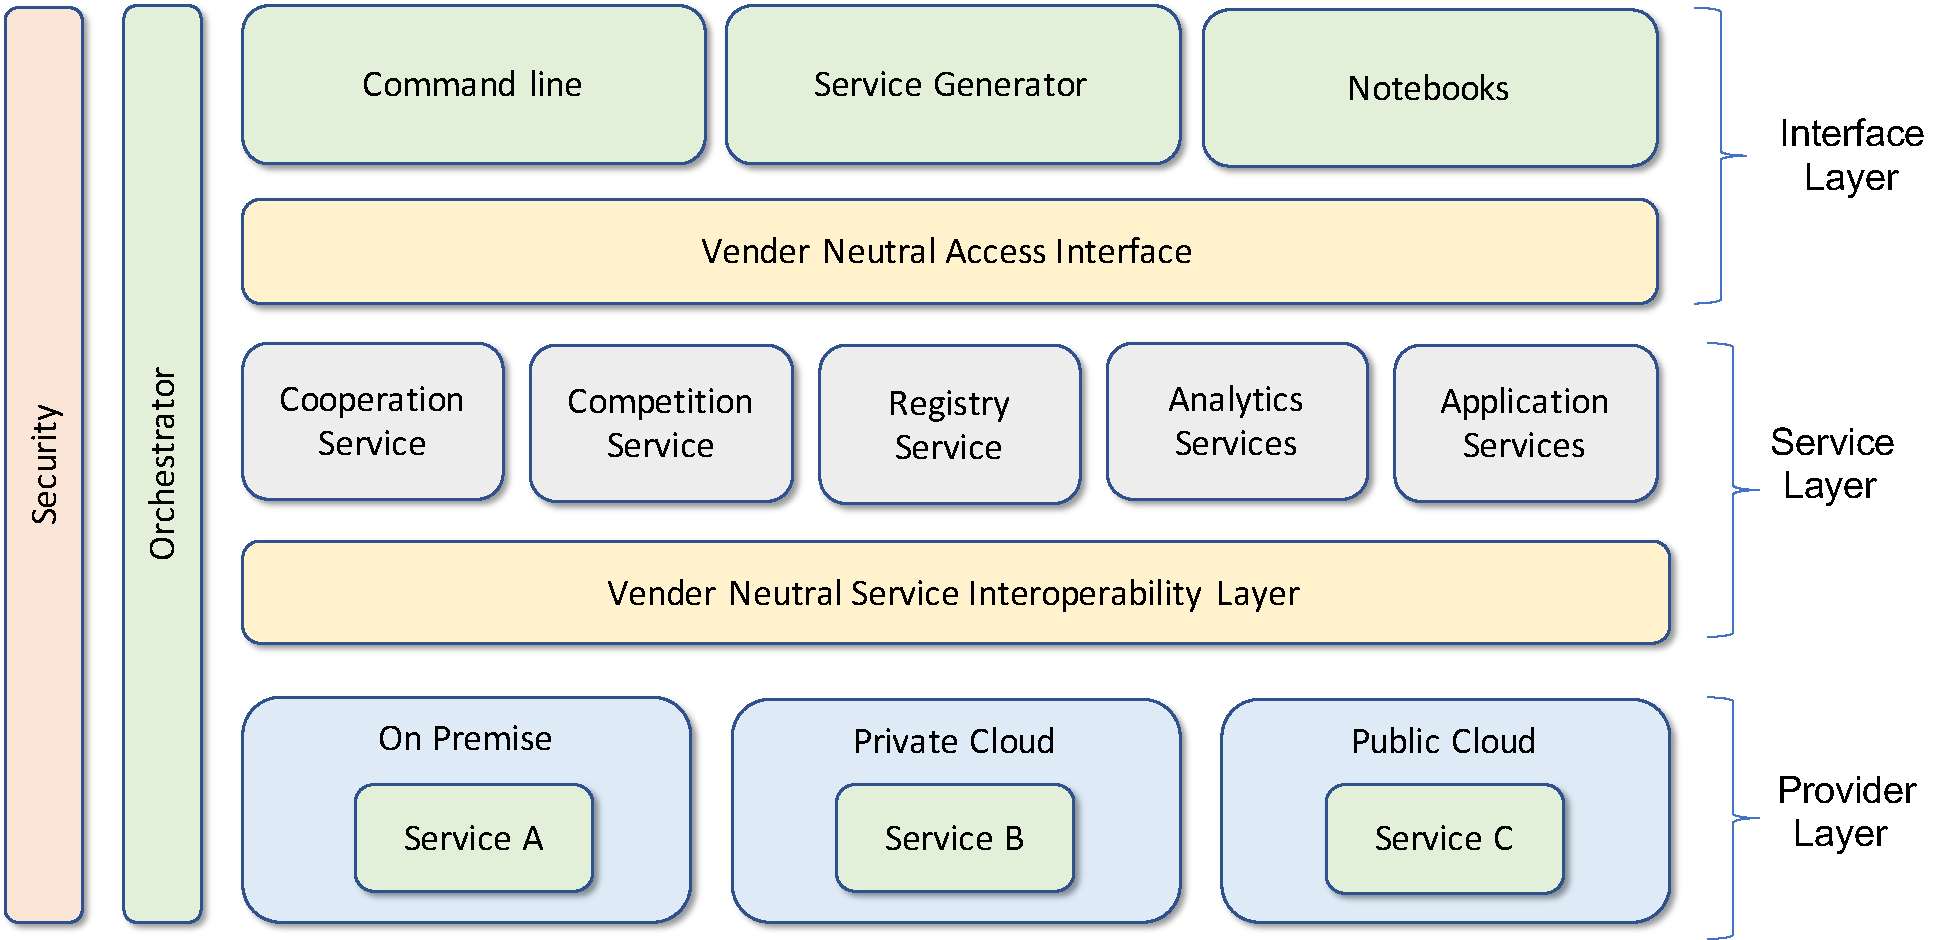
\includegraphics[width=1.0\columnwidth]{images/hybrid-service-arch.pdf}
    \end{center}
  \caption {Architecture of the hybrid multi-analytics service
    framework}
  \label{fig:arch}
\end{figure}

The architecture is organized in layers  and contains
multiple components in each layer. We distinguish the interface,
service, and provider layer. Security and an orchestration service
enable the integration of the various components into a coordinated
application pipeline.

\subsection{Interface Layer}

Today's analytics is invoked through a multitude of interfaces, making
it possible to invoke them in different languages, but also high level
frameworks. This is often achieved by an interface layer using REST
to communicate with the other layers. For our work, we focus on
the command line interface promoting reuse in shells, Jupyter notebooks
showcasing the reuse in an interactive analysis capable framework, and
our previous work to generate REST services (see Section \ref{s:gas}).

\subsubsection{Command Line Interface}

To provide reusability within the DevOps application of data analytics
pipelines, we provide an enhanced command-line interface that
specifically targets hybrid and multi-analytics environments. This is
facilitated by adding command options, shell variables, and
configuration files that can be passed into the commands.
Most importantly, we analyze which specific parameters we
need to make available when investigating cooperative and competitive
services. The parameters can be directly translated to REST service invocations.

\subsubsection{Interactive Notebooks}

Although it is important to provide a command-line interface that can
easily be used to generate computing activities for solving data
analytics tasks, it is even more critical that the framework can be
integrated into interactive steering tasks conducted directly by the
data scientists. For this, we leverage Jupyter notebooks and integrate
service calls to the backend system into the notebooks just as we can
in regular python programs. The difference here is that Jupyter
provides a rich set of interactive components and widgets that can be
leveraged to prototype interactive services but also parameter
studies. While our
previous work has been integrated into notebooks, the capabilities of
notebooks were not yet fully utilized as the integration was done on
the service level but not on a level where Jupyter was used to enhance
the service pipeline. 

\subsection {Service Layer}

\subsubsection{Generalized Analytics Services}
\label{s:gas}

While we have focused previously on the automated generation of
services using REST, we need to consider the other aspects of this
architecture that is needed to support the data analyst. We have
shown that it is possible to create rest services from Python
functions and classes while augmenting them with helper services such
as data uploads. The development of such services is out of the
capability of many data scientists as they focus on developing
transformative data analysis functions and not on the infrastructure
service generation. Our work is lowering the bar for such
implementation and allowing even data analysts to generate reusable
REST services \cite{las21openapi}. The effort to learn how to
create vendor-independent and computer language-independent services
has been reduced from months to days. We can leverage this effort to
generate application-specific services quickly. The services generated
are integrated into a user-managed service registry. We leverage
this service and enabled its exposure via REST through FastAPI as part
of the generator.

\subsubsection{Hybrid Multi-Analytics Service Registry}

% \TODO{Gregor: rewrite}

While we have previously developed a simplified generalized service
registry, we are exploring significant extensions to integrate (a)
container images, (b) container services, and (c) analytics 
services offered by service providers. This registry is specially
designed to support cooperating and competing for analytics services.
We intend to add the ability to leverage existing repositories, such as
GitHub and DockerHub to register suitable analytics services as source
code. We will then also add features to provide endpoints to
instantiated services so they can be advertised to a large group of
users. A neutral vendor specification is used as part of the
registry. Such a registry can be hosted by a user or an
organization. We will identify if it is possible to leverage GitHub
for hosting such a registry. This will require a special set of tools
and programs to keep the registry up to date. A user can then
integrate such a registry into their analytics pipeline. New analytics
service specifications can then be either integrated through direct
specifications added to the hosted registry or through the use of
GitHub submodules. Using submodules offers the ability to keep up to
date with analytics services developed by others and allows updates
through automated DevOps-controlled pull requests. This registry
technology would completely replace our earlier registry work if
successful. It would also allow the integration of private services as
private analytics services can be integrated while using private
submodules hosted in private repositories. Hence, the details of such
modules are not exposed. As GitHub also supports GraphQL we will
explore using GraphQL as a mechanism for the specification of Registry
entries. To increase privacy, git can also be hosted on-premise.

\subsection{Application Services}

An application may require the availability of very specific
application-oriented analytics services. Our architecture allows us to
integrate them while reusing the same vendor-neutral specification
format. This includes not only cloud services but also the
integration of analytics services that rely on on-premise
infrastructure. An example would be access to a supercomputer in the
TOP500 list that is used to conduct a complex data analytics task
reusing GPUs to conduct deep learning for COVID-19 analysis. This
results in two specifications. A general specification that can be
reused on other similar on-premise computers, and a second that is
specifically targeted to the targeted on-premise infrastructure. This
could include the integration of hosted data services or specific
network capabilities.

\subsection{Analytics Services}

Data analysts are developing analytics functions on a regular
basis. As we can use our service generator to transform them into
analytics services, we will be able to create and register them into
our registry. We will expand upon our available services but focus on
services that explicitly address multi-cloud and hybrid service use
cases.

A good example may be natural language processing to analyze a text
with either a local service, a loud hosted service by different
vendors. Here, based on input parameters, we create an overarching
language analytics service that chooses the various services with the
the help of service level requirements and agreements.

\subsection{Cooperation and Competition Services}

As previously indicated, we already have identified two special use
cases of data analytics services that leverage hybrid and
multi-analytics 
services. This is the specification of services that
employ:


\paragraph{Cooperation.} Cooperating services are services that use one or
more services from hybrid multi-analytics services. They are
cooperating together to address the solution to a formidable data
analytics problem. Thus the resources form a "team" of services that
work together. This includes the integration of specialized services
that may not be unique to a particular provider. Still, it also could
mean that computational analytics processes could be performed in
parallel, and results could be gathered to accelerate the analytics
task. A parameter study is a very good example of one kind of
cooperating services

\paragraph{Competition.} Here, the available hybrid multi-analytics services
directly compete with each other. This can be done by direct selection
of services that are more suitable than others. This selection could
be based on resource requirements such as time, availability, cost,
and feature. However, the framework could take "observations" and
propose automated conclusions about which services to choose from. A
possibility would even be to integrate deep-learning strategies into
the selection process.
  

\subsection{Provider Layer}

An integral part of the proposal is identifying how we can leverage
services from multiple providers, including on-premise services. We
have shown in our previous work that we can specify vendor-neutral
specifications to access, for example, virtual machines. We will expand
this concept while using the concept of containers. However, we also
need to identify services that are offered by
multiple vendors, such as language processing services. Although they
can be directly accessed via vendor-specific interfaces. It will
be important to identify if they can be generalized so the users
can benefit from a uniform vendor-neutral service interoperability
layer. We will identify a usability example to explore the
possibilities of this approach.

\subsection{Crosscutting Services}

We have two crosscutting services. One is the {\em orchestrator} that
allows the specification of service pipelines to combine the various
services that are needed for application implementation. The other
is a {\em security} service that will enable us to access the various services
through the required authentication and authorization mechanisms. The
latter we have demonstrated in {\em cloudmesh} where users can manage their
own access to a multi-cloud environment ta access their activated
analytics services. We will leverage from that effort but  also leverage from
open source solutions that can be embedded in our vendor-neutral
service specification, such as basic and OAUTH security. In general, we
abstract the security calls to be callouts to the appropriate
authentication mechanisms.

